\newpage
\section{Grundlagen}\label{Grundlagen}
Fehlender-Text

\subsection{Service Roboter}
In den letzten Jahren haben Service Roboter in verschiedenen Branchen an Bedeutung gewonnen. Ein Grund hierfür ist der technische Fortschritt der Robotik, KI, Big Data, Kameras, Sensoren und Spracherkennung \cite[S.~424]{Paluch2020}. Dieser Abschnitt gibt einen kurzen Überblick über Service Roboter im allgemeinen und eine Einführung in die Funktionen der Roboter, die in dieser Arbeit eingesetzt werden. Auch wird das System beschrieben, über das der Prototyp mit den Robotern kommuniziert.

\subsubsection{Definition}
In wissenschaftlichen Arbeiten wird mit vielen verschiedenen Definitionen für Service Roboter gearbeitet. In dieser Arbeit wird die Definition aus der ISO Norm 8373:2021 \cite[Kap.~3]{ISO2021} verwendet. Nach dieser handelt es sich bei Service Robotern um Roboter die im privaten oder professionellen Gebrauch nützliche Aufgaben für Menschen erledigen. Hierbei werden Service Roboter von Industrierobotern und Medizinrobotern abgegrenzt. Die \ac{IFR} \cite{IFR2024} ergänzt die Voraussetzung, dass Service Roboter voll- oder zumindest teilautonom handeln können. Unter professionellem Gebrauch versteht man den kommerziellen Einsatz \cite[S.~4]{GonzalezAguirre2021}, unter anderem im Gesundheitswesen, in der Landwirtschaft und im Tourismus \cite[S.~9]{GonzalezAguirre2021}.

\subsubsection{Einsatzmöglichkeiten}
Service Roboter werden bereits in vielen Bereichen eingesetzt. So gibt es verschiedene Beispiele in denen Service Roboter in Hotels für den Gästeempfang, Check-in und Gepäcklieferung eingesetzt werden. Auch werden Sie an Flughäfen für die Beratung von Reisenden, Scannen von Boardingpässen, Check-in, Bodenreinigung und Patrouilliengänge genutzt. In der Pflege helfen Service Roboter den Pflegern beim Heben von Patienten und durchführen von Übungen mit Patientengruppen. Auch können Roboter in der Pflege angenehme Gespräche starten \cite[S.~425-427]{Paluch2020}. Aufgaben mit geringer kognitiver und emotionaler Komplexität können Service Roboter hierbei vollautonom und ohne Aufsicht durch einen Menschen durchführen \cite[S.~429]{Paluch2020}. Hierbei handelt es sich beispielsweise um Aufgaben wie Staubsaugen, Rasenmähen oder Gepäcklieferung. Für komplexere Aufgaben braucht es die Aufsicht oder Unterstützung von Menschen, wodurch diese nur teilautonom ausgeführt werden.

Service Roboter, die im Kontakt mit Kunden eingesetzt werden, bieten verschiedene mögliche Vorteile, die aber immer abgewägt werden müssen. Beispielsweise können Roboter Emotionen vorspielen, die von Kunden aber als unauthentisch erkannt werden. Dafür können Roboter durchgängig freundlich sein und können nicht so wie Menschen unter emotionalem Burnout leiden \cite[S.~427]{Paluch2020}. 

\subsubsection{Pudu Robotics}
% TODO erwähnen das Roboter eine eingestellte Ladestation haben.
Wie erwähnt, beschäftigt sich diese Arbeit mit Robotern von Pudu. Pudu stellt Service Roboter her, die vor allem für verschiedene Zwecke in der Gastronomie eingesetzt werden können. Die Modelle sind hierbei auf unterschiedliche Funktionen, wie das Begrüßen von Gästen, das Liefern bestellter Speisen und Getränke, das Zurückbringen dreckigen Geschirs und das Putzen des Bodens spezialisiert \cite{PUDU2024}.

Damit die Roboter diese Funktionen ausführen können, müssen sie eigenständig durch komplexe, sich ändernde Umgebungen navigieren können. Das eigenständige Navigieren lässt sich in die Teilfunktionen die Positionsfindung, Wahrnehmung und Routenplanung aufteilen, wobei die Positionsfindung eine Schlüsselrolle spielt \cite{Nature2022}. Zur Positionsfindung erstellen sich die Roboter mit \ac{VSLAM} eine Karte ihrer Umgebung. Bei einer Fläche von 1000 Quadratmetern kann das eine Stunde dauern. Während Roboter normalerweise platzierte Markierungen brauchen, können sich die Pudu Roboter mithilfe einer nach oben gerichteten Kamera an der Zimmerdecke orientieren.\cite{Pudu2023} Durch weitere Kameras und Sensoren können die Pudu Roboter ihre Umgebung wahrnehmen\cite{Nature2022}.

\subsubsection{Bot Control Backend}\label{sec:BotControlBackend}
Im Rahmen dieser Arbeit wird eine bereits existierende Schnittstelle zwischen den Pudu Robotern und der prototypischen Webanwendung genutzt. Diese Schnittstelle ist das sogenannte \ac{BCB}. In diesem Abschnitt wird die Kommunikation zwischen dem \ac{BCB} und den Pudu Robotern erläutert. Die folgenden Informationen zum Service Framework von Pudu, das zur Kommunikation zwischen Robotern und \ac{BCB} genutzt wird, stammen aus dem SDK Guidance Document von Pudu \cite{PuduSDK}. Das Dokument steht nicht im Internet zur Verfügung und bietet keine genaueren Informationen zur MQTT basierten Kommunikation zwischen Microservice, PUDU Cloud und Robotern.

Die Abbildung \ref{fig:BotControlBackendCommunication} veranschaulicht die Kommunikation zwischen dem \ac{BCB} und den Robotern. Wie man in der Abbildung sieht hat das \ac{BCB} nur eine direkte Verbindung zum Node.js Microservice, welches wiederum über die PUDU Cloud mit den Robotern kommuniziert. Über \gls{HTTP}-Anfragen an den Microservice können Befehle verschickt und Daten abgefragt werden. Die Anfragen werden vom Microservice via \gls{MQTT} an die PUDU Cloud weitergeleitet. Anfragen die nicht an die Roboter weitergeleitet werden müssen, weil die angefragten Daten in der PUDU Cloud liegen, werden auf dem gleichen Weg direkt beantwortet. Muss mit den Robotern kommuniziert werden, dann wird die Anfrage von der PUDU Cloud über \gls{MQTT} an die relevanten Roboter weitergeleitet, die diese dann beantworten. Die Roboter können auch unaufgefordert Ereignisse an das \ac{BCB} kommunizieren. Hierfür muss das \ac{BCB} eine Adresse für einen bestimmten Ereignistyp im Microservice als \gls{Webhook} registrieren. Tritt das entsprechende Ereignis auf, schickt der Roboter diese Information via \gls{MQTT} über die PUDU Cloud an den Microservice. Dieser schickt daraufhin eine HTTP-Anfrage an die registrierte Adresse im \ac{BCB}.

\begin{figure}[H]
\caption{Kommunikation zwischen Bot Control Backend und Robotern}\label{fig:BotControlBackendCommunication}
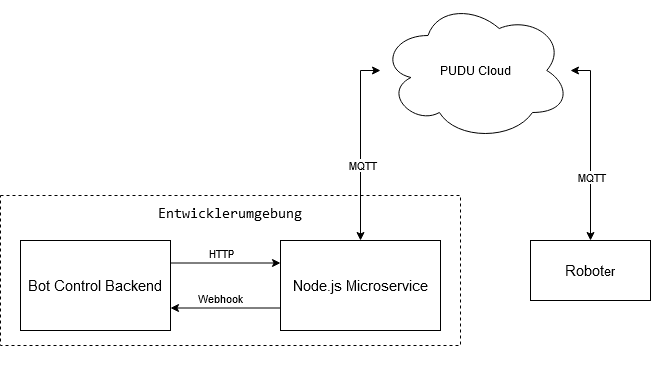
\includegraphics[width=0.9\textwidth]{BotControlBackend Diagramm}
\\
Quelle: In Anlehnung an Pudu \cite[S.~4]{PuduSDK}
\end{figure}

Das \ac{BCB} dient nicht nur als Schnittstelle zu den Pudu Robotern, sondern abstraiert auch neue Funktionen aus denen die Pudu bietet. Zum können Roboter durch das \ac{BCB} über einen Fahrstuhl zu einem Lieferpunkt in einem anderen Stockwerk fahren. Zum anderen kann der Roboter vor einer geschlossenen Tür halten, diese öffnen und dann weiter fahren. Es gibt verschiedene Daten, die von den Robotern abgerufen werden und relevant für den Prototyp sind. So gibt es die Roboterposition in Relation zur mit \ac{VSLAM} generierten Karte. Zudem gibt es die Positionen der relevanten Standorte wie Lieferpunkte und Ladestation. Neben diesen Positionen gibt es zudem die Pfade, an denen sich die Roboter bei der Fahrt orientieren und virtuelle Wände, die manuell platziert werden müssen, damit bestimmte Bereiche nicht durchfahren werden. Beispielsweise ergibt es Sinn, Treppen als virtuelle Wände zu markieren, damit diese nicht versehentlich angefahren werden.

\subsection{Webanwendungen}
% Plattformunabhängigkeit mit Quelle erwähnen
Fehlender-Text

\subsubsection{Technologien und Softwarebibliotheken}\label{sec:WebTechnologies}
TODO: HTML erklären; Typescript und Javascript erklären; SCSS und CSS erklären; React erklären; React Redux erklären; Deployment erklären.

\subsubsection{chayns}\label{sec:Chayns}
TODO: chayns-Seite erläutern; chayns-Application erläutern; UAC-Gruppen erläutern; Admin-Modus erläutern; npx create-chayns-app; chayns-components; chayns-api; chayns.space erläutern; websocket-service erwähnen.

\subsection{3D Modelle}
Dieser Abschnitt bietet eine kurze Einführung in 3D-Modelle. Daraufhin werden verschiedene Methoden zur Erzeugung von 3D-Gebäudemodellen vorgestellt. Abschließend wird erläutert, wie 3D-Modelle in Webanwendungen eingebunden werden können.

3D-Modelle sind digitale Darstellungen von Objekten oder Szenen in drei Dimensionen. Anders als bei herkömmlichen 2D-Grafiken, die lediglich Breite und Höhe haben, enthalten 3D-Modelle zusätzlich Tiefeninformationen. Polygonale 3D-Modelle bestehen aus Polygonen, die sich aus Eckpunkten und Verbindungen zwischen Eckpunkten in der Form von Kanten zusammensetzen. Oberflächeneigenschaften der Polygone, wie Farbe, Glanz und Reflexionen lassen sich durch die Anwendung von Texturen und Materialien definieren. Transformationsoperationen wie Skalierung, Rotation und Translation ermöglichen es, 3D-Modelle im Raum zu bewegen und zu manipulieren. Kameras, Perspektiven und Projektionen den Betrachterstandpunkt und die Darstellung des Modells festlegen.\cite[S.~8-16]{Parisi2014}

\subsubsection{Generierung}
Neben der manuellen Modellierung von 3D-Modellen mithilfe von Modellierungssoftware wie Blender gibt es verschiedene Methoden, die sich insbesondere zur Generierung von Raummodellen eignen.

\paragraph{Fotogrammetrie}

Die Fotogrammetrie beschäftigt sich damit Messungen aus einer Vielzahl an zweidimensonalen Bildern abzuleiten und mit diesen präzise 3D-Modelle zu erzeugen\cite[S.~19]{Aber2010}. Inzwischen erfordert Fotogrammetrie nicht mehr den Einsatz teurer Kameras, da die Kameras moderner Mobilgeräte eine ausreichende Bildqualität bieten\cite{Cohrs2021}. Der Prozess der Fotogrammetrie lässt sich in mehrere Schritte gliedern. Zunächst braucht es eine sorgfältige Planung der Aufnahmen. Hierbei sollte auf eine gleichmäßige Belichtung geachtet werden. Außerdem sollten innerhalb der Szene reflektierende und transparenten Flächen sowie jegliche Bewegung von Objekten vermieden werden. Während der Aufnahme müssen Parameter wie Belichtungszeit und Weißabgleich passend konfiguriert sein, wobei diese Einstellungen zwischen den einzelnen Aufnahmen unverändert bleiben sollten. Des Weiteren ist darauf zu achten, dass sich der Inhalt aufeinanderfolgender Bilder stets überschneidet.\cite{Cohrs2021b} Zum Schluss erfolgt die Verarbeitung der Aufnahmen mithilfe spezialisierter Software, deren Bedienung komplex sein kann. Für eine reibungslose Verarbeitung sind eine leistungsstarke Grafikkarte und ausreichend Speicherplatz unerlässlich.\cite{Cohrs2021c}

\paragraph{LiDAR Scanning}
Im Gegensatz zur Fotogrammetrie nutzt \ac{LiDAR} einen aktiven Sensor. Dabei wird Licht in Form eines pulsierenden Lasers ausgesendet. Das reflektierte Licht wird darufhin mit einem Scanner erfasst, wodurch die Berechnung von Distanzen zu Punkten ermöglicht wird. Auf deren Grundlage wird dann ein 3D-Modell erstellt. Seit 2020 werden LiDAR-Scanner in neuere iOS-Geräte von Apple integriert, in der Hoffnung eine verbesserte Bildqualität zu ermöglichen\cite{Fenstermaker2022}. Als Nebeneffekt wurden verschiedene Apps entwickelt, die den LiDAR-Scanner nutzen, um 3D-Modelle zu erstellen, wie zum Beispiel Canvas\cite{Canvas2023}, Polycam\cite{Polycam2024} und Scaniverse\cite{Scaniverse2024}. Diese Apps versprechen eine einfache Generierung von 3D-Modellen.

\paragraph{KI gestützte Methoden}
Es existieren verschiedene KI-Modelle, die darauf trainiert sind, ein 3D-Gebäudemodell mit nur wenigen Bildern zu erzeugen. Eines dieser Modelle ist Plan2Scene. Es benötigt einen Grundriss des Gebäudes als Eingabe sowie Bilder, die den einzelnen Räumen zugeordnet sind. Basierend auf dem Grundriss generiert das Modell ein 3D-Modell mit Möbeln. Basierend auf den Bildern der Räume werden monotone Texturen für Wände und Böden generiert.\cite[S.~10733]{Plan2Scene2021} Das Rent3D Modell funktioniert ähnlich, generiert aber keine Texturen für Wände und Böden und nutzt stattdessen die Bildaufnahmen selbst als Textur\cite[S.~3413]{Rent3D2015}.

\subsubsection{Einbindung im Web}
Die Einbindung von 3D-Modellen wird im Web durch \ac{WebGL} und WebGPU ermöglicht. Während \ac{WebGL} für lange Zeit der etablierte Standard war, gewinnt WebGPU seit der Veröffentlichung im Jahr 2021 stetig an Popularität.

\paragraph{WebGL}
\ac{WebGL} wurde 2011 von der Khronos Group entwickelt und ist eine Javascript-API mit der 3D-Grafiken im Webbrowser ohne zusätzliche Plugins dargestellt werden können. Die 3D-Grafiken können hierbei hardwarebeschleunigt, also über den Einsatz spezialisierter Hardware - wie einer \ac{GPU} - angezeigt werden. Hierdurch wird eine hohe Leistungsfähigkeit ermöglicht, solange ein Gerät Hardwarebeschleunigung unterstützt. Durch die Integration mit HTML und Javascript können 3D-Grafiken dynamisch in Webseiten eingebunden werden. Da \ac{WebGL} auf offenen Webstandards basiert, ist es in allen Browsern plattformunabhängig sowohl an Desktop- als auch an Mobilgeräten nutzbar.\cite[S.~17-19]{Parisi2014} WebGPU bietet wie WebGL das hardwarebeschleunigte Anzeigen von 3D-Grafiken und darüber hinaus eine verbesserte Leistung sowie erweiterte Funktionen\cite{Surma2022}. Entwicklern steht eine Vielzahl an Frameworks zur Verfügung die auf \ac{WebGL} oder WebGPU basieren\cite{Seguin2024} und die Entwicklung im Vergleich zu diesen vereinfachen und beschleunigen.

\paragraph{\deckgl{}}
Das Framework \deckgl{} wurde 2016 von Uber als Open Source Projekt veröffentlicht\cite{Visgl}. Das Framework basiert auf \ac{WebGL}, wobei ab der kommenden Version 9.0.0 stattdessen WebGPU eingesetzt werden soll\cite{Green2022}. Mit \deckgl lassen sich hochperformante interaktive Karten und Geovisualisierungen mit tausenden bis millionen Datenpunkten im Web einbinden. Da das Framework auf React ähnlichen Programmierparadigmen basiert eignet es sich besonders gut für die Einbindung in React Anwendungen. Das Framework funktioniert nach dem \ac{PIL} Paradigma. So werden Datenpunkte gruppiert in einer Ebene dargestellt, die mindestens ein grundlegendes visuelles Element nutzt. So kann es sich bei diesen grundlegenden Elementen um Kreise, Rechtecke und Linien aber auch komplexere teilweise auch dreidimensonale Elemente handeln. Diese Elemente werden innerhalb der Ebene auf Basis der Datenpunkte und deren Attribute positioniert, skaliert und gefärbt. Die Ebenen können gestapelt und somit kombiniert werden, was auch die Inspiration für den Namen des Frameworks ist, da im Englischen deck of cards Kartenstapel bedeutet.\cite[S.~2]{YangWang2019} Das Framework bietet verschiedene vordefinierte Ebenen, wie die IconLayer \cite{DeckglIconLayer}, die Bilder als das grundlegende visuelle Element nutzt. So kann kann einem Datenpunkt ein Bild an der passenden Position zugewiesen werden. In dem Beispiel aus Abbildung \ref{fig:IconLayerExample} wird die IconLayer - in Kombination mit einer Basisebene zur Darstellung der Weltkarte - genutzt um die Positionen aller bekannten Meteoritenlandungen auf der Erde anzuzeigen.

\begin{figure}[H]
    \caption{IconLayer Beispiel}\label{fig:IconLayerExample}
    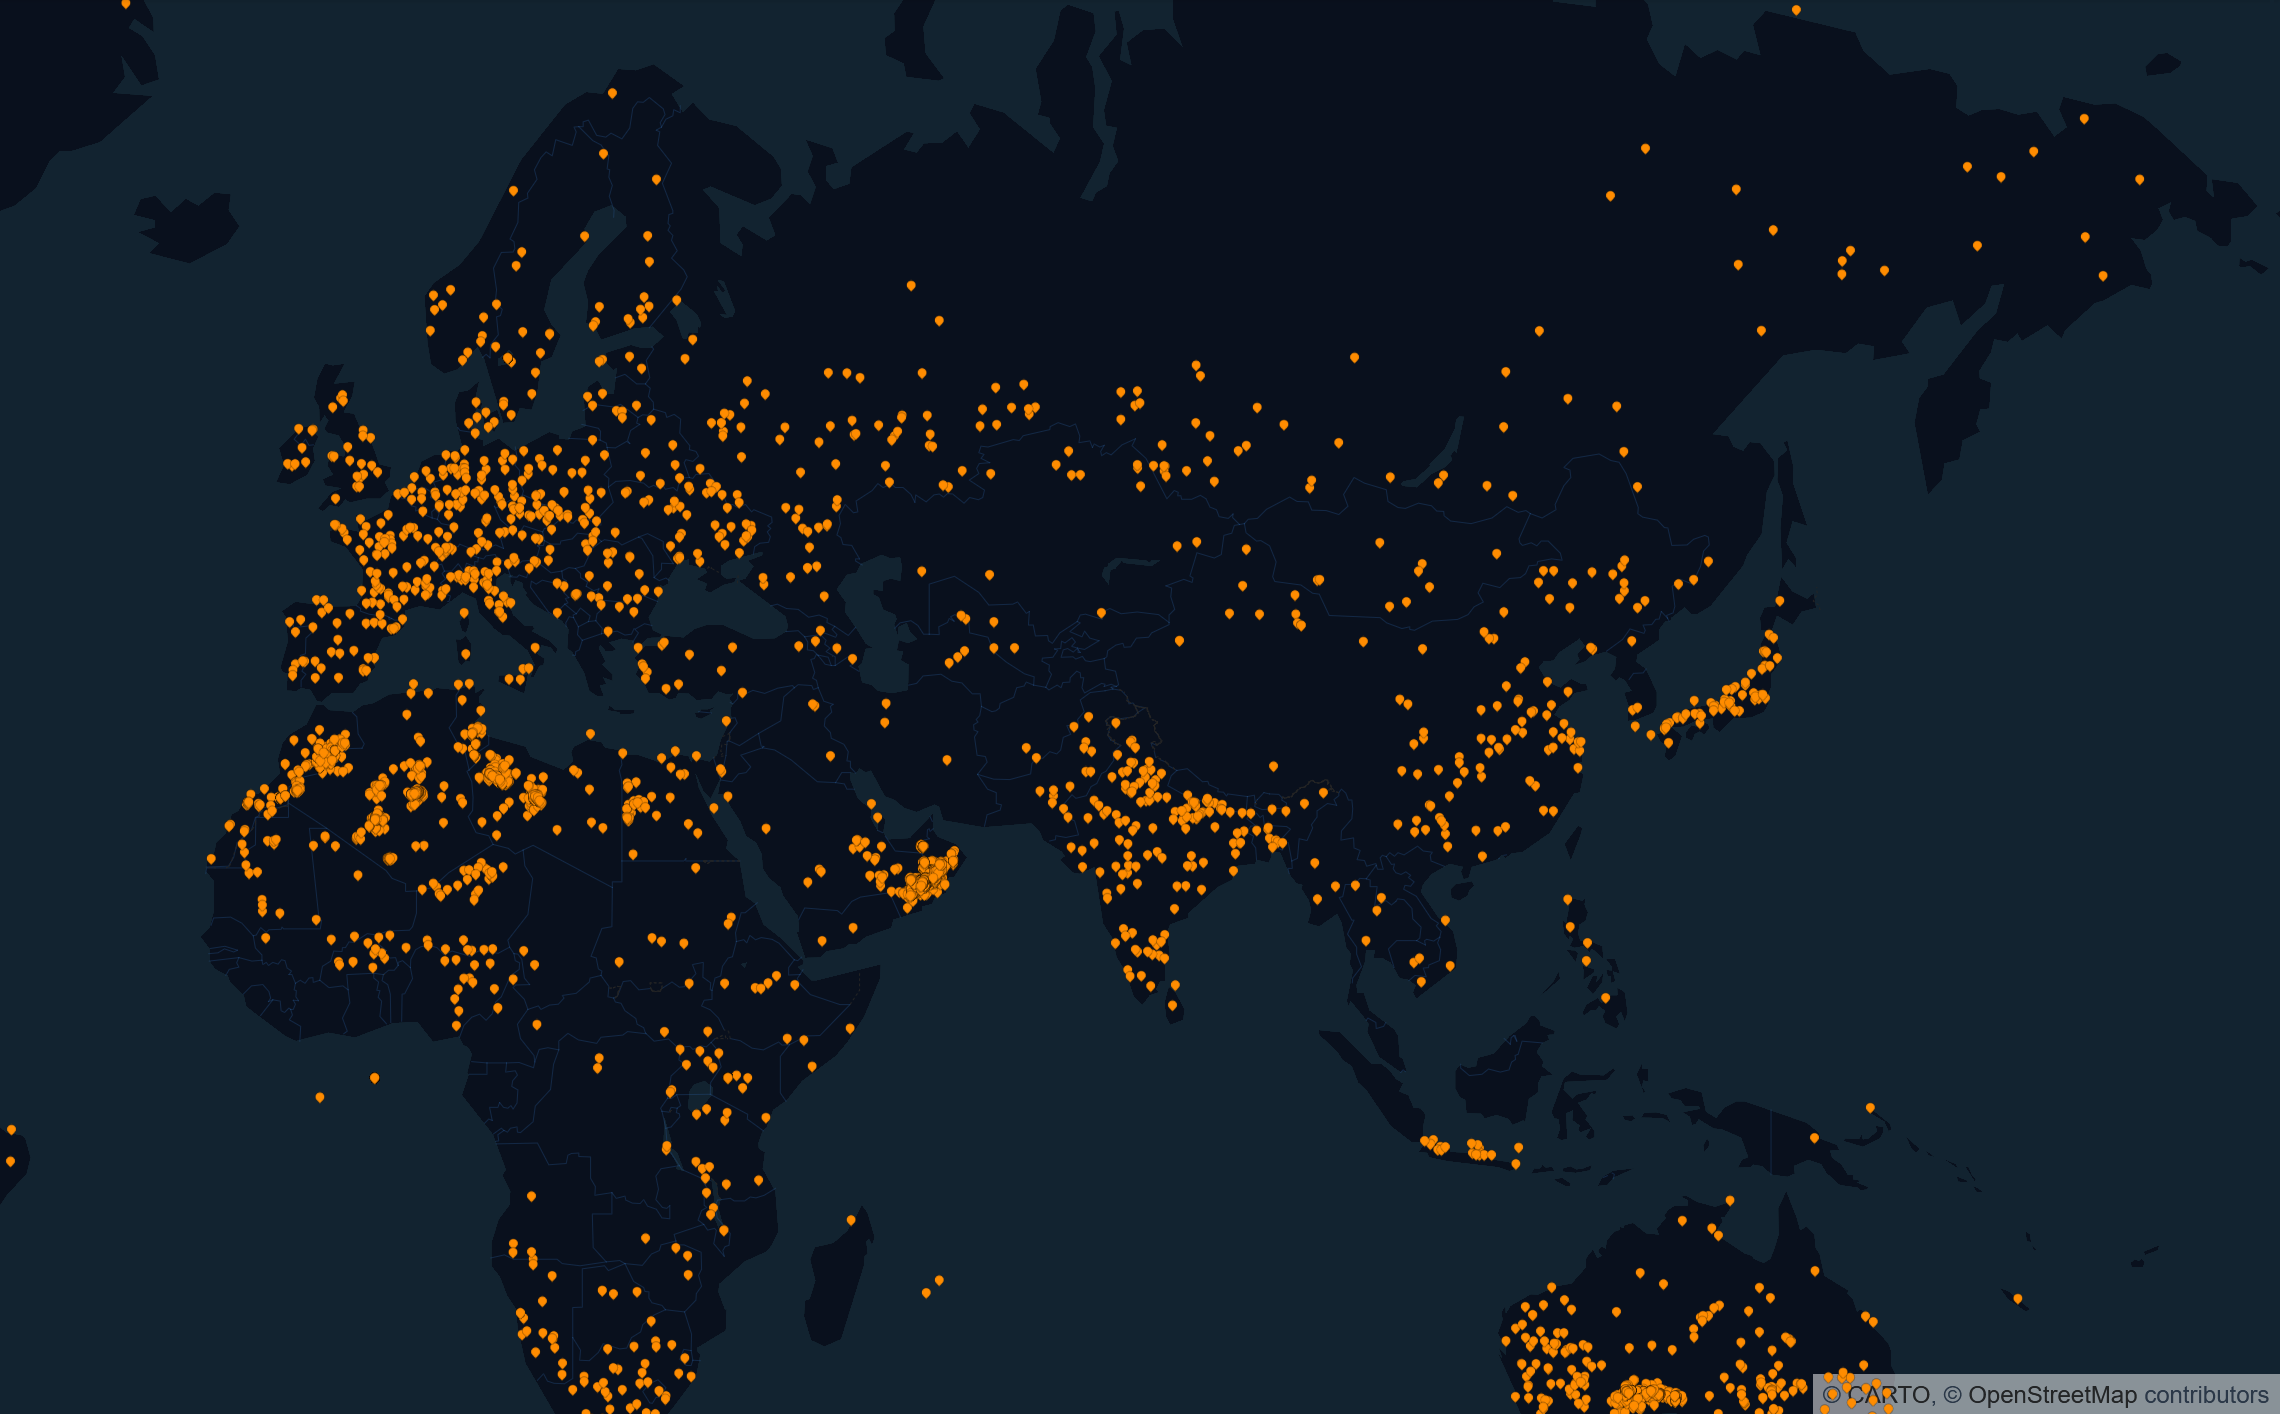
\includegraphics[width=0.9\textwidth]{IconLayer Example.png}
    \\
    Quelle: OpenJS Foundation \cite{DeckGlMeteorites}
\end{figure}

Weitere für diese Arbeit relevante vordefinierte Ebenen sind die SimpleMeshLayer \cite{DeckglSimpleMeshLayer} und ScenegraphLayer \cite{DeckglScenegraphLayer} für die Anzeige von 3D-Modellen und die PathLayer für das Anzeigen von Pfaden. Es können auch neue Ebenen entwickelt werden, was für diese Arbeit aber nicht relevant ist, da die Auswahl an vordefinierten Ebenen ausreicht. Weitere wichtige Elemente die \deckgl{} bietet sind die Controller Klasse \cite{DeckglController}, mit der die Navigation auf der Karte konfiguriert werden kann und die Viewport Klasse \cite{DeckglViewport} mit der die Navigation direkt gesteuert werden kann.

\subsection{Softwarequalität}
"Unter Softwarequalität versteht man die Gesamtheit der Merkmale und Merkmalswerte eines Softwareprodukts, die sich auf dessen Eignung beziehen, festgelegte oder vorausgesetzte Erfordernisse zu erfüllen" \cite[S.~257]{Balzert1998}. So ergibt sich die Softwarequalität aus der Erfüllung der definierten Anforderungen und Erwartungen und zielt darauf ab den Bedürfnissen der Benutzer gerecht zu werden. Für die Bestimmung der Softwarequalität gibt es verschiedene Merkmale die ausgewertet werden können. Nach dem ISO-Standard ISO/IEC 25010 gibt es acht Produktqualitätsmerkmale \cite{ISO25010}, die auch in der Abbildung \ref{fig:SoftwareQuality} aufgelistet sind. Die Merkmale Effizienz und Benutzbarkeit haben Relevanz für diese Arbeit, da diese direkt durch die Forschungsfrage gefordert werden und auch die funktionale Eignung ist relevant, da diese die Erfüllung der funktionalen Anforderungen abdeckt, die in Kapitel \ref{sec:FunctionalRequirements} definiert werden. Währenddessen haben die restlichen Mekrmale weniger Releavanz, da im Rahmen dieser Arbeit nur ein Prototyp entwickelt wird, der nicht die Ansprüche an ein Produktivsystem erfüllen muss. Im Folgenden werden die drei relevanten Merkmale genauer erläutert.
% TODO Quelle ISO 25010

\begin{figure}[H]
    \caption{Qualitätsmerkmale}\label{fig:SoftwareQuality}
    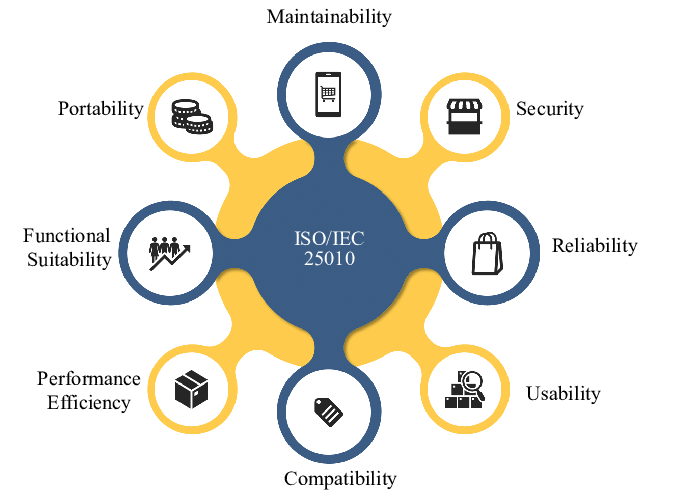
\includegraphics[width=0.9\textwidth]{Qualitaetsmerkmale.png}
    \\
    Quelle: TODO
\end{figure}
% TODO Quelle hinzufügen

\subsubsection{Benutzbarkeit}
Die Benutzbarkeit wird nach ISO 25010 in sechs Kriterien aufgeteilt: angemessene Erkennbarkeit, Erlernbarkeit, Bedienbarkeit, Toleranz gegenüber Anwenderfehlern, Ästhetik der Benutzeroberfläche und Barrierefreiheit.
% TODO Quelle ISO 25010
Mithilfe dieser Merkmale soll bewertet werden können wie einfach und angenehm ein Produkt für einen Nutzer zu bedienen ist.

\paragraph{Usability Heuristics}
Die zehn Usability Heuristics von Nielsen sind grundlegende Richtlinien zur Bewertung der Benutzerfreundlichkeit von Softwareprodukten und Websites. Während der Entwicklung können diesen Richtlinien berücksichtigt werden, um die Benutzerfreundlichkeit zu verbessern. Bis auf die Barrierefreiheit decken die Usability Heuristics alle Kriterien der Benutzbarkeit nach ISO 25010 ab. Zwei der Usability Heuristics sind die Übereinstimmung zwischen dem System und der realen Welt, um die Lernkurve zu reduzieren und die Einhaltung von Konsistenz und Standards, damit Elemente möglichst selbsterklärend sind.
% TODO Quelle Usability Heuristics
Eine subjektive Bewertung der Einhaltung dieser Richtlinien durch die Entwickler ist unzureichend um die Benutzerfreundlichkeit zu bewerten. Stattdessen eignet sich hier ein Expertenreview oder Usability Tests besser.

\paragraph{Usability Tests}
Usability Tests werden durchgeführt, damit die Benutzerfreundlichkeit eines Produkts bewertet werden kann. Hierfür werden Testpersonen bei der Nutzung des Produkts beobachtet. Die Testpersonen spielen hierbei zuvor entwickelte Anwendungsszenarien durch. Bei den Testpersonen sollte es sich um potenzielle Benutzer des Produkts handeln.\cite[S.~22]{Dumas.1999}. Nach der Durchführung der Tests werden die gesammelten Beobachtungen auf Probleme und Schwachstellen im Produkt ausgewertet. Die Tests können entweder quanitativ oder qualitativ durchgeführt werden. Bei quantitativen Usability Tests werden verschiedene Metriken, wie die Durchführungszeit oder die Rate der erfolgreichen Durchführung von Aufgaben gesammelt.
Mit Usability Tests lässt sich die Benutzerfreundlichkeit eines Produkts bewerten, indem Benutzer bei der Nutzung beobachtet werden und diese Beobachtungen. Diese Metriken zeigen im Vergleich zu den Ergebnissen früherer oder zukünftiger Tests, wie sich die Benutzerfreundlichkeit mit der Zeit entwickelt hat. Bei qualitativen Usability Tests werden Testpersonen bei der Interaktion mit dem Produkt beobachtet, wodurch sich Designmerkmale identifizieren lassen, die gut oder schlecht zu bedienen sind.\cite{Budiu.2017}. Qualitative Tests brauen einen Moderator, der die Testpersonen durch den Testprozess leitet. Gegebenenfalls gibt es auch weitere Beobachter, die nicht mit den Testpersonen interagieren.\cite{Moran.2019} Für qualitative Tests reicht eine Auswahl von fünf Testpersonen aus, um einen Großteil der Probleme zu finden. Mit einer zunehmenden Menge an Testpersonen sinkt das Return of Investment maßgeblich dadurch, dass immer weniger neue Fehler pro Testperson entdeckt werden.\cite{Nielsen.2012}

\subsubsection{Performance}

\subsubsection{Softwaretest}